\chapter{背景介绍}


模型检测将待检测的系统建模为一个跃迁系统(transition system),在时序逻辑(temporal logic)中指定待验证的属性。给定模型\(M\) 和属性\(\varphi\),模型检测将验证是否\(M\)满足\(\varphi\)。在不同的模型检测方法中,高级符号模型检查(Advanced Symbolic Model Checking)\citep{Grobelna_2015}使用简化的有序二叉决策图(Reduced Ordered Binary Decision Diagrams,ROBDDs 或 BDDs)\citep{Bryant_1986}来表示状态集合和转移关系。通过迭代调用图像计算算法来计算所有可达状态,判断一个模型是否满足时间属性,直到达到不动点为止。

最近,随着量子计算的发展,关于量子线路的验证技术也在不断发展\citep{viamontes2007checking,burgholzer2020advanced}。其中,利用模型检测方法对线路进行自动化验证也有了一些应用。由于量子线路运算空间随着量子比特的线性增加而指数级膨胀,传统的计算方法并不能很好应对。因此本次研究希望应用基于张量网络(tensor network)的张量决策图(tensor decision diagrams)进行量子模型检测。

而在本章中将简要介绍本次研究中的一些重要的基础知识。因此本章分为两节。第一节介绍量子计算相关背景,包括量子力学和量子线路。第二节介绍模型检测相关背景,包括跃迁系统,时序逻辑和量子模型检测。
\section{量子计算简介}
% //TODO:add more intro
量子计算机(quantum computer)是一种利用量子比特特性进行计算的一种设备。在量子计算中,量子比特的特殊性质允许其同时处于多种状态,这与经典比特的二进制状态不同。量子计算机的状态空间可以用希尔伯特空间(Hilbert space)\(\mathcal{H}\)表示\citep{nielsen2010quantum},即可以进行内积运算(inner product)的复向量空间。比特状态可以用\(\mathcal{H}\)的向量表示,量子门由\(\mathcal{H}\)上的酉算子(unitary operator)表示。

量子线路(quantum circuit)是一种描述量子计算的模型。在量子线路中,通过量子比特的初始化、应用量子门、测量以及其他可能的操作的序列来构建和执行量子计算任务。量子线路通常从左向右阅读,每个量子门的作用是将输入的量子比特状态转变为输出状态,该过程可以认为是量子门的酉矩阵与输入的量子状态的乘积。
\begin{figure}[!htbp]
    \centering
    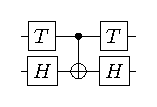
\includegraphics[width=.6\textwidth]{Img/example_cir.pdf}
    \caption{一个量子线路的例子}
    \label{fig:example_cir}
\end{figure}

图\ref{fig:example_cir} 所示的量子线路展示了一个具体的量子线路示例。其中有单比特门\(H=\frac{1}{\sqrt2}\left[\begin{matrix}1&1\\1&-1\\\end{matrix}\right],T=\left[\begin{matrix}1&0\\0&e^{-i\pi/4}\\\end{matrix}\right]\),以及双比特门\(CX=\left[\begin{matrix}\begin{matrix}1&0\\0&1\\\end{matrix}&\begin{matrix}0&0\\0&0\\\end{matrix}\\\begin{matrix}0&0\\0&0\\\end{matrix}&\begin{matrix}0&1\\1&0\\\end{matrix}\\\end{matrix}\right]\)。假设该量子线路的初始状态为\(\left|\psi\right\rangle=\left|\psi_1\right\rangle\left|\psi_2\right\rangle\),则输出状态为\(T\otimes H\cdot CX\cdot T\otimes H\cdot\left|\psi\right\rangle\)。

在量子计算机上可以执行各种算法和计算任务,如量子搜索\citep{Grover_1996}、量子因子分解\citep{Shor}和量子模拟\citep{Feynman}等。量子计算的潜力在于其能够在某些特定问题上比经典计算机更高效地进行计算,尤其在处理大规模数据和解决复杂问题方面具有潜在优势。本节对该部分进行简单介绍,而需要对这部分深入了解的读者,可以自行阅读\citep{nielsen2010quantum}。

\subsection{量子力学}
量子力学有两种主要的表述:波动力学和矩阵力学。其中波动力学由Erwin Schrödinger首创,矩阵力学由Werner Heisenberg首创。波动力学使用微分方程为数学基础,更接近于经典物理的波动理论,适用于处理时间演化问题和连续系统。
而矩阵力学使用线性代数为数学基础,适用于具有离散能级的系统。由于在量子计算中,大量使用矩阵力学作为理论基础。
因此本小节主要介绍矩阵力学。
\subsubsection*{线性代数}
线性代数的基本研究对象是向量空间(vector space),也称作线性空间(Linear Spaces)。这是一种抽象的数学结构,用于描述向量的集合。向量空间在向量加法(Vector Addition)和标量乘法(scalar multiplication)封闭。
对于一个向量空间,向量的类型满足特定条件。向量可以是几何向量、函数、多项式或任何满足向量空间公理的对象。
同时还需要定义标量域(Scalars)\(\mathbb{F}\) ,在大多数情况下,标量是实数(Real Numbers)\(\mathbb{R}\)或复数(Complex Numbers)\(\mathbb{C}\),用于通过标量乘法运算改变向量的大小。
最后向量空间的还需要遵循一系列公理。这些公理规定了向量加法和标量乘法的性质,如加法的交换律和结合律、加法和标量乘法的分配律、加法单位元的存在性(即零向量,Zero Vector),以及乘法单位元(即标量1)的存在性。这些公理确保了向量空间内运算的一致性和预测性。

此外子空间(Subspace)也是是向量空间中的一个重要概念。子空间指的是一个向量空间的一个子集,同时它自身也是一个向量空间。因此子空间遵循向量空间的向量加法和标量乘法运算封闭的性质。线性算子 (Linear Operator),也称为线性映射(Linear Mapping)或线性变换(Linear Transformation),是在向量空间中的一种特殊函数,它在两个向量空间之间映射向量,保持向量加法和标量乘法的结构。% 线性算子定义
设 \(V\) 和 \(W\) 是两个向量空间,一个线性算子 \(T: V \rightarrow W\) 必须满足以下两个条件:
\begin{enumerate}
    \item 加法性 (Additivity):对于所有 \(u, v \in V\),有 \(T(u + v) = T(u) + T(v)\)。
    \item 齐次性 (Homogeneity):对于所有标量 \(a \in \mathbb{F}\) 和所有 \(v \in V\),有 \(T(av) = aT(v)\)。
\end{enumerate}
当$T$是\(T: W \rightarrow W\)的线性算子,则$T$是定义在向量空间$W$上的线性算子。其中恒等算子(identity operator)$T$是向量空间$W$上的线性算子,满足以下条件:
\begin{align}
    T(w) = w,\forall w \in W
\end{align}

此外有的向量空间还有内积和张量积(Tensor product)操作。内积定义为:\(( \cdot, \cdot ): V \times V \rightarrow \mathbb{F}\),其中 $V$ 是一个向量空间。对于任意两个向量 $u$ 和 $v$,它们的内积 $( u, v )$ 满足以下性质:
\begin{enumerate}
    \item 共轭对称性(Conjugate Symmetry): \(( u, v ) = \overline{( v, u )}\),其中\(\overline{( v, u )}\)是\(( v, u )\)的复共轭,当标量域为实数时,表现为对称性,即\(( u, v ) = ( v, u )\)
    \item 线性 (Linearity)或齐次性:\(( \alpha u_1 + \beta u_2, v ) = \alpha( u_1, v ) + \beta( u_2, v )\),其中\(\alpha,\beta\in\mathbb{F}\)
    \item 正定性 (Positive Definiteness):\(( v, v ) \geq 0\)且仅当\(v \)为加法单位元时等号成立
\end{enumerate}
% 张量积定义
可以看到内积是一种特殊形式的线性算子。而张量积则提供了一种方法来构造新的向量空间。
设 \(V\) 和 \(W\) 是两个向量空间,它们的张量积 \(V \otimes W\) 是一个新的向量空间,满足以下性质:
\begin{enumerate}
    \item 对于每一对元素 \(v \in V\) 和 \(w \in W\),存在一个元素 \(v \otimes w \in V \otimes W\),称为它们的张量积。
    \item 张量积满足双线性性(Bilinearity):对于所有 \(v,v' \in V\),\(w,w' \in W\) 以及所有标量 \(a,b \in \mathbb{F}\),有
    \[
    (av + bv') \otimes w = a(v \otimes w) + b(v' \otimes w),
    \]
    \[
    v \otimes (aw + bw') = a(v \otimes w) + b(v \otimes w').
    \]
    \item 张量积是唯一的,意味着对于任何与 \(V \otimes W\) 具有相同性质的向量空间,都存在一个自然同构映射(Natural Isomorphism)到 \(V \otimes W\)。
\end{enumerate}

矩阵力学的数学基础建立在希尔伯特空间\(\mathcal{H}\),即一个可以进行内积运算的复向量空间。
希尔伯特空间中的向量由复数\(n\)元组\(\left(c_1,c_2,\cdots,c_n\right)\)构成,可以记作\(\mathbb{C}^n\),其中\(c\)表示复数。向量也可以有以下列矩阵形式:
\begin{align}
    \left[\begin{matrix}
        c_1\\c_2\\\vdots\\c_n
    \end{matrix}\right]
\end{align}
\(\mathbb{C}^n\)中的标量为复数。因此可以定义\(\mathbb{C}^n\)矩阵形式的标量乘法运算为:
\begin{align}
    c'\left[\begin{matrix}
        c_1\\c_2\\\vdots\\c_n
    \end{matrix}\right]=\left[\begin{matrix}
        c'\cdot c_1\\c'\cdot c_2\\\vdots\\c'\cdot c_n
    \end{matrix}\right]
\end{align}
其中等式右边的乘法为复数乘法,因此复数1为乘法单位元。类似地,\(\mathbb{C}^n\)矩阵形式的向量加法可以定义为:
\begin{align}
    \left[\begin{matrix}
        c_1\\c_2\\\vdots\\c_n
    \end{matrix}\right]
    +\left[\begin{matrix}
        c'_1\\c'_2\\\vdots\\c'_n
    \end{matrix}\right]=\left[\begin{matrix}
        c_1+c'_1\\c_2+c'_2\\\vdots\\c_n+c'_n
    \end{matrix}\right]
\end{align}
其中等式右边的乘法为复数加法,因此零向量的矩阵形式如下:
\begin{align}
    \left[\begin{matrix}
        0\\0\\\vdots\\0
    \end{matrix}\right]
\end{align}
通常将该向量记作\(\mathbf{0}\)。

类似地,可以定义\(\mathbb{C}^n\)矩阵形式的内积和张量积运算为:
\begin{align}
    \left(\left[\begin{matrix}
        c_1\\c_2\\\vdots\\c_n
    \end{matrix}\right]
    ,\left[\begin{matrix}
        c'_1\\c'_2\\\vdots\\c'_n
    \end{matrix}\right]\right)=
    \sum_{i=1}^{n}c_i^* c'_i
\end{align}
\begin{align}
    \left[\begin{matrix}
        c_1\\c_2\\\vdots\\c_n
    \end{matrix}\right]
    \otimes\left[\begin{matrix}
        c'_1\\c'_2\\\vdots\\c'_n
    \end{matrix}\right]=\left[\begin{matrix}
        c_1c'_1\\c_1c'_2\\\vdots\\c_1c'_n\\c_2c'_1\\\vdots\\c_n c'_n
    \end{matrix}\right]
\end{align}
在量子计算中,通常将向量\(\psi\)记作狄拉克右矢符号\(|\psi\rangle\)。
对向量\(|\psi\rangle\)中的复数全部取共轭,可以得到\(|\psi\rangle\)的共轭记作\(|\psi\rangle^*\)。
向量\(|\psi\rangle\)的共轭转置可以记作\(|\psi\rangle^\dagger\),也称对偶向量,可以用狄拉克左矢符号\(\langle\psi|\)表示。因此向量之间的内积也可以用以下方法表示:
\begin{align}
    (|\psi\rangle, |\phi\rangle)=\langle \psi|\phi\rangle , \forall |\psi \rangle, |\phi \rangle\in \mathcal{H}
\end{align}

希尔伯特空间\(\mathcal{H}\)中的线性算子集合,通常记作\(\mathcal{L} (\mathcal{H})\)。
对算子\(A \in \mathcal{L}\),$A$的伴随算子(adjoint operator)$A^\dagger$定义为:
\begin{align}
    \langle \psi |A^\dagger|\phi \rangle = \langle \phi |A|\psi \rangle^*, \forall |\psi \rangle, |\phi \rangle\in \mathcal{H}
\end{align}
算子\(A \in \mathcal{L}\),被称为作Hermite算子(Hermite operator),或者Hermitian,当且仅当满足以下条件:
\begin{align}
    A = A^\dagger
\end{align}


如果一个Hermitian算子\(A\)同时满足:
\begin{align}
    A^2 = A
\end{align}
那么\(A\)也被称作投影算子(project oroperator)。

如果一个Hermitian算子\(A\)同时满足:
\begin{align}
    A^\dagger A = A A^\dagger
\end{align}
那么\(A\)也被称作正规算子(normal oroperator)。同时\(A\)是正规算子,当且仅当被如下对角化:
\begin{align}
    A = \sum_{i}\lambda_i |i\rangle\langle i|
\end{align}
其中$\lambda_i$是$A$的特征值,$|i\rangle$为对应特征值的特征向量。

如果一个Hermitian算子\(A\)同时满足:
\begin{align}
    A^\dagger A = I
\end{align}
其中$I$表示希尔伯特空间中的恒等算子。那么\(A\)也被称作酉算子(unitary oroperator)。
酉算子保持向量之间的内积,即:
\begin{align}
    (U|\psi\rangle, U|\phi\rangle) = \langle \psi|U^\dagger U|\phi\rangle = \langle \psi|I|\phi\rangle = \langle \psi|\phi\rangle = (|\psi\rangle, |\phi\rangle), \forall |\psi \rangle, |\phi \rangle\in \mathcal{H}
\end{align}
\subsubsection*{量子力学基本假设}
在量子力学中,有四条基本假设,其数学框架是在不断实验中总结,假设,验证而得到的。
\begin{theorem}
    任何量子系统都可以用一个带内积的复向量空间表示,即希尔伯特空
    间,称为系统的状态空间(state space)。量子系统可由该空间的单位向量描述,这
    些向量被称为状态向量(state vector)。
\end{theorem}
\begin{theorem}
    一个封闭的量子系统(closed quantum system)的演化(evolution) 可以由酉算子(unitary operation) 表示。
\end{theorem}
常见算子的矩阵形式
\begin{theorem}
    量子测量(quantum measurement) 由一组测量算子 (measurement opera
    tor) $M_m$ 刻画,这些算子作用在被测量的量子系统的状态空间上。其中下标$m$
   对应测量后可能得到的测量结果。
\end{theorem}
\begin{theorem}
    复合系统(composite system) 的状态空间是其各个子空间的状态空间的
    张量积。如果复合系统从$1$到$n$的子系统,并且第$i$个系统的状态为$|\psi_i\rangle$。则复合系统的状态为\(|\psi_1\rangle\otimes|\psi_2\rangle\otimes\cdots\otimes |\psi_n\rangle\)。
\end{theorem}
\subsection{量子线路}

\section{模型检测简介}
\textcolor{red}{写一点导语}
\subsection{跃迁系统}
跃迁系统广泛应用于模型检测中待检测系统的建模,其定义为\citep{baier2008principles}:
\begin{equation}
\mathcal{M}=\{S,Act,\rightarrow,I\}
\end{equation}
其中\(S\)为系统状态集合,\(I\)为系统初态集合,因此满足\(I\subseteq S\)。\(Act\)为系统行为集合。\(\rightarrow\)为系统状态转移关系,即\(\rightarrow\subset S\times Act\times S\)。此外还有\(AP\)为描述系统原子命题。L是标记函数,将状态映射为状态满足的原子命题集合。需要验证的属性\(\varphi\)将表述为命题。


系统的有限路径片段\(\pi\)是一个有限状态序列\(s_0,s_1\ldots s_n\)。\(s_i\)满足\(s_{i-1}\overset{a}{\rightarrow}s_i,a\in Act\),对于所有\(0<i\leq n\),其中\(n\geq 0 \)。无限路径片段\(\pi\)是一个无限状态序列\(s_0,s_1\ldots\),使得对于所有\(i>0\),\(s_{i-1} \overset{a}{\rightarrow}  s_i,a\in Act\)。在路径中\(\pi\left[i\right]=s_i,\pi\left[i\right)=s_i\ldots\)。所有以\(s_0\)为开始的路径,构成了路径集合\(Path\left(s_0\right)\)。

\begin{figure}[!htbp]
    \centering
    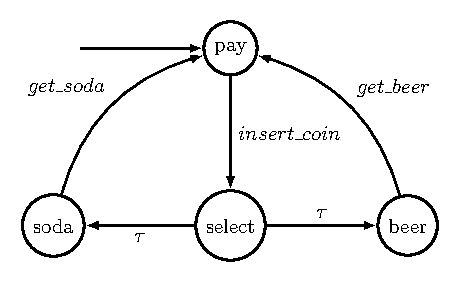
\includegraphics[width=.6\textwidth]{Img/map.pdf}
    \caption{一种简化版的售货机跃迁系统}
    \label{fig:transition-system}
\end{figure}

图\ref{fig:transition-system} 所示的跃迁系统展示了一个简化版的售货机模型。在该模型中,用户投入硬币,进行选择后就可以得到苏打水或者啤酒。在该例子中,系统状态\(S=\{pay,select,soda,beer\}\),系统初态\(I=pay\)。
系统行为\(Act=\{insert\_coin,\tau,get\_soda,get\_beer\}\),其中\(\tau\)表示立即行动符号。转移关系图中已经展示。原子命题可取\(AP=\{paid,drink\}\)。因此\(L\left( pay \right)=\{\varnothing\}\),\(L\left(soda\right)=L\left(beer\right)=\{paid,drink\}\),\(L\left(select\right)=\{paid\}\)。系统的一个路径是\(\pi=pay\ select\ soda\ pay\ selsect\ \ldots\)。此时\(\pi\left[1\right]=slect,\pi\left[1\right)=select\quad soda\quad pay\quad selsect\ldots\)。同时该路径满足\(\pi\in Path\left(pay\right)\)。
量子模型检测的跃迁系统类似。区别在于状态空间用\(\mathcal{H}\),转移关系用酉矩阵。一个量子自动机定义如下:
\begin{align}
    \mathcal{M}=\{\mathcal{H},Act,\{U_\alpha,\alpha\in Act\},\mathcal{H}_0\}
\end{align}
下面介绍模型检测中的使用的时序逻辑。

\subsection{时序逻辑的验证}
在量子模型检测中,与经典模型检测一样使用时序逻辑指定待验证的属性\(\varphi\)。时序逻辑命题的运算符有两类\citep{goranko_2023}。状态命题公式(State formulas):\(\varphi ::=a\left|\exists\varphi\right|\forall \varphi\left|\lnot\varphi\right|\varphi\land\psi\),其中\(a\in AP\)。以及路径命题公式(Path formulas):\(\varphi\Colon=O\varphi|\varphi U\psi\)。给定模型的一个状态为\(s\),路径为\(\pi\),则具体满足条件分别如下:
\begin{itemize}
    \item \(s\models a,iff \L\left(s\right)\models a\)
    \item \(s\models\exists\varphi,iff\ \pi\models\varphi\)对一些\(\pi\in Path\left(s\right)\)
    \item \(s\models\forall\varphi,iff\ \pi\models\varphi\)对所有\(π\in Paths\)
    \item \(s\models\lnot\varphi,iff\ s\nvDash\varphi\)
    \item \(s\models\varphi\land\psi,iff\ s\models\varphi\ and\ s\models\psi\)
    \item \(\pi\models O\varphi,iff\ \pi\left[1\right]\models\varphi\)
    \item \(\pi\models\varphi U\psi,iff\ \exists j\geq0\).\(\pi\left[j\right)\models\psi\) 同时对所有\(0\le i<j\)有\(\pi\left[i\right)\models\varphi\)
\end{itemize}


图\ref{fig:path-formula-basic} 展示了两种路径命题公式的直观示意图。


\begin{figure}[!htbp]
    \centering
    \begin{subfigure}[b]{0.8\textwidth}
        \centering
        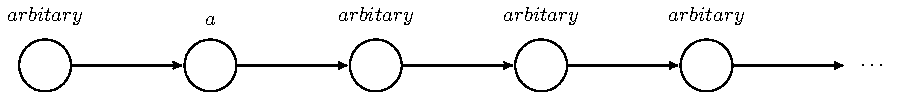
\includegraphics[width=\textwidth]{Img/path_for_Oa.pdf}
    \end{subfigure}
    \\
    \begin{subfigure}{0.8\textwidth}
        \centering
        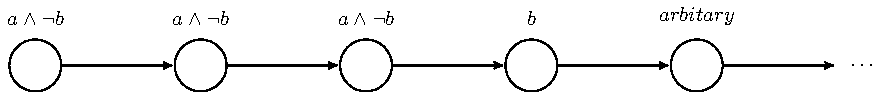
\includegraphics[width=\textwidth]{Img/path_for_aUb.pdf}
    \end{subfigure}
    \caption{$\pi\models O a $与 $\pi\models a U b$的图示}
    \label{fig:path-formula-basic}
\end{figure}
在模型检测中,有三类比较重要的可达性问题,分别是可达性、持续可达性以及重复可达性。过程中主要涉及以下路径命题公式:\(\lozenge\) 表示最终(eventually),\(\square\)表示总是(always),\(\lozenge\square\)表示总是最终(always eventually),\(\square\lozenge\)表示最终总是(eventually always)。其中\(\lozenge\)和\(\square\)具体定义为:
\begin{itemize}
    \item \(\lozenge\varphi\overset{\text{def} }{=} \text{True}U\varphi\)
    \item \(\square\varphi\overset{\text{def} }{=} \neg\lozenge\neg\varphi\)
\end{itemize}
图\ref{fig:path-formula}展示了这两种基本路径命题公式的直观示意图。
\begin{figure}[!htbp]
    \centering
    \begin{subfigure}[b]{0.8\textwidth}
        \centering
        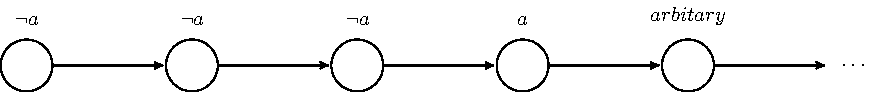
\includegraphics[width=\textwidth]{Img/path_for_Dia.pdf}
    \end{subfigure}
    \\
    \begin{subfigure}{0.8\textwidth}
        \centering
        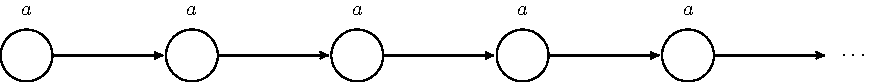
\includegraphics[width=\textwidth]{Img/path_for_SQa.pdf}
    \end{subfigure}
    \caption{$\pi\models\lozenge a$与 $\pi\models\square a$的图示}
    \label{fig:path-formula}
\end{figure}

具体的可满足条件为:
\begin{itemize}
    \item \(\pi\models\lozenge\varphi,iff\exists j\ge0.\pi[j)\models\varphi\)
    \item \(\pi\models\square\varphi,iff\forall j\ge 0.\pi[j)\models\varphi\)
    \item \(\pi\models\lozenge\square\varphi,iff\exists i\ge 0.\forall j\ge i,\pi[j)\models\varphi\)
    \item \(\pi\models\square\lozenge\varphi,iff\forall i\ge 0.\exists j\ge i,\pi[j)\models\varphi\)
\end{itemize}
基于此三种可达性问题定义分别如下:
\begin{itemize}
    \item 可达性:\( Pr^{\mathcal{M}}(s \models \lozenge G) = Pr^M(\pi \models \lozenge G : \pi \in \text{Paths}(s))\)
    \item 持续可达性:\( Pr^{\mathcal{M}}(s \models \lozenge \square G) = Pr^M(\pi \models \lozenge \square G : \pi \in \text{Paths}(s))\)
    \item 重复可达性:\( Pr^{\mathcal{M}}(s \models\square \lozenge G) = Pr^M(\pi \models \square\lozenge G : \pi \in \text{Paths}(s))\)
\end{itemize}
\subsection{量子模型检测}
目前量子的模型检测,主要使用Birkhoff-von Neumann Quantum Logic来描述量子系统的性质\citep{birkhoff1987logic}。Birkhoff-von Neumann量子逻辑是一种非经典逻辑,用于描述量子力学中事件的逻辑结构。它由 Birkhoff 和 von Neumann 在 1936 年首次提出。在量子逻辑中,命题的集合不再形成布尔代数,而是形成一个投影算子的正交完备格,这与传统的逻辑系统不同。

在 Birkhoff-von Neumann 量子逻辑中,量子系统的状态可以由希尔伯特空间(Hilbert space)来描述,每个量子命题对应希尔伯特空间的一个闭子空间。对于系统的状态 \(|\psi\rangle\),如果它属于某个特定的闭子空间 \( \mathcal{X} \),我们可以说这个命题是真的。

例如,考虑以下量子逻辑命题:

\begin{itemize}
\item 命题 \( \mathcal{X} \):在时间 \( t \) 时,量子粒子的位置 \( x \) 坐标在区间 \( [a, b] \) 内。
\item 命题 \( \mathcal{Y} \):在时间 \( t \) 时,量子粒子的动量 \( y \) 坐标在区间 \( [a, b] \) 内。
\end{itemize}

这些命题 \( \mathcal{X} \) 和 \( \mathcal{Y} \) 可以通过粒子的状态希尔伯特空间的特定子空间来表示。

在数学上,这种逻辑结构可以使用格理论(lattice theory)来描述,其中格中的元素对应于量子事件,格的操作则对应于逻辑运算。在确定了原子命题后,需要引入连接词,这些连接词可以用来构建更复杂的命题,以描述量子系统的复杂属性。在语义上,这些可以被视为在希尔伯特空间$\mathcal{H}$的一个子空间 \(S(\mathcal{H})\) 中的代数操作。
具体如下:
\begin{itemize}
    \item 子空间之间的包含关系 \( \subseteq \) 在 \(S(\mathcal{H})\) 中是一个偏序关系,它可以理解为量子逻辑的蕴含(元逻辑)。
    \item 一个子空间 \( \mathcal{X} \) 的正交补 \( \mathcal{X}^\perp \) 在量子逻辑中用作否定的解释。
    \item \(S(\mathcal{H})\) 对交集是封闭的,即对于 \(S(\mathcal{H})\) 中的任何元素族 \( \{\mathcal{X}_i\} \),都有$\bigcap_{i} \mathcal{X}_{i} \in \mathcal{S}(\mathcal{H})$。在量子逻辑中用于表示合取。
    \item 对于一组子空间 \(\{\mathcal{X}_i\}\),它们的并集定义为
    \(
    \bigvee_i \mathcal{X}_i = \text{span} \left( \bigcup_i \mathcal{X}_i \right).
    \)
    。在量子逻辑中,析取被解释为并集。
\end{itemize}

\( (S(\mathcal{H}), \cap, \vee, \perp) \) 构成一个正交模糊格,\( \subseteq \) 是其排序,这是 Birkhoff–von Neumann 量子逻辑的代数模型。

在实际应用中,通常只选择 \( S(\mathcal{H}) \) 的一个子集 AP 作为原子命题的集合。AP 中的元素可以被认为是真正关心的那些命题,而其他的可能是不相关的。出于算法目的,通常假设 AP 是可数的甚至是有限的 \( S(\mathcal{H}) \) 的子集,而不是 \( S(\mathcal{H}) \) 本身,因为 \( S(\mathcal{H}) \) 是不可数无限的。因此给定一组原子命题集 AP,对于 \( \mathcal{X} \in S(\mathcal{H}) \),如果状态 \(|\psi\rangle\) 满足集合中所有命题的交集,我们说 \(|\psi\rangle\) 满足 \(\mathcal{X}\)。需要对这部分深入了解的读者,可以自行阅读\citep{2021}。


% //TODO: modify structure. here is the backgroud
